%%% The main file. It contains definitions of basic parameters and includes all other parts.

%% Settings for single-side (simplex) printing
% Margins: left 40mm, right 25mm, top and bottom 25mm
% (but beware, LaTeX adds 1in implicitly)
\documentclass[12pt,a4paper]{report}
\setlength\textwidth{145mm}
\setlength\textheight{247mm}
\setlength\oddsidemargin{15mm}
\setlength\evensidemargin{15mm}
\setlength\topmargin{0mm}
\setlength\headsep{0mm}
\setlength\headheight{0mm}
% \openright makes the following text appear on a right-hand page
\let\openright=\clearpage

%% Settings for two-sided (duplex) printing
% \documentclass[12pt,a4paper,twoside,openright]{report}
% \setlength\textwidth{145mm}
% \setlength\textheight{247mm}
% \setlength\oddsidemargin{14.2mm}
% \setlength\evensidemargin{0mm}
% \setlength\topmargin{0mm}
% \setlength\headsep{0mm}
% \setlength\headheight{0mm}
% \let\openright=\cleardoublepage

%% Generate PDF/A-2u
\usepackage[a-2u]{pdfx}

%% Character encoding: usually latin2, cp1250 or utf8:
\usepackage[utf8]{inputenc}

%% Prefer Latin Modern fonts
\usepackage{lmodern}

%% Further useful packages (included in most LaTeX distributions)
\usepackage{amsmath}        % extensions for typesetting of math
\usepackage{amsfonts}       % math fonts
\usepackage{amsthm}         % theorems, definitions, etc.
\usepackage{bm}             % boldface symbols (\bm)
\usepackage{graphicx}       % embedding of pictures
\usepackage{fancyvrb}       % improved verbatim environment
\usepackage{natbib}         % citation style AUTHOR (YEAR), or AUTHOR [NUMBER]
\usepackage[nottoc]{tocbibind} % makes sure that bibliography and the lists
			    % of figures/tables are included in the table
			    % of contents
\usepackage{dcolumn}        % improved alignment of table columns
\usepackage{booktabs}       % improved horizontal lines in tables
\usepackage{paralist}       % improved enumerate and itemize
\usepackage{xcolor}         % typesetting in color
\usepackage{url}
\usepackage{verbatim}
%%% Basic information on the thesis

\usepackage{acronym}
\usepackage{makecell}
\usepackage{listings}
\usepackage{enumitem}
\usepackage{bbding}
% \usepackage[nobottomtitles]{titlesec}
\newcommand\short{}

\newcommand{\emptyline}{\vspace{\baselineskip}}

% Thesis title in English (exactly as in the formal assignment)
\def\ThesisTitle{Declarative Web Automation Toolkit}

% Author of the thesis
\def\ThesisAuthor{Jindřich Bär}

% Year when the thesis is submitted
\def\YearSubmitted{2022}

% Name of the department or institute where the work was officially assigned
% (according to the Organizational Structure of MFF UK in English,
% or a full name of a department outside MFF)
\def\Department{Department of Software Engineering}

% Is it a department (katedra), or an institute (ústav)?
\def\DeptType{Department}

% Thesis supervisor: name, surname, and titles
\def\Supervisor{RNDr. Jakub Klímek, Ph.D.}

% Supervisor's department (again according to Organizational structure of MFF)
\def\SupervisorsDepartment{Department of Software Engineering}

% Study programme and specialization
\def\StudyProgramme{Computer Science}
\def\StudyBranch{Databases and Web}

% An optional dedication: you can thank whomever you wish (your supervisor,
% consultant, a person who lent the software, etc.)
\def\Dedication{%
Dedication.
}

% Abstract (recommended length around 80-200 words; this is not a copy of your thesis assignment!)
\def\Abstract{%
Abstract.
}

% 3 to 5 keywords (recommended), each enclosed in curly braces
\def\Keywords{%
{web} {automation} {scraper} {crawler} {declarative programming}
}

%% The hyperref package for clickable links in PDF and also for storing
%% metadata to PDF (including the table of contents).
%% Most settings are pre-set by the pdfx package.
\hypersetup{unicode}
\hypersetup{breaklinks=true}

% Definitions of macros (see description inside)
\include{macros}

% Title page and various mandatory informational pages
\begin{document}

\unless\ifdefined\short
	\include{title}

	%%% A page with an automatically generated table of contents of the bachelor thesis
\fi

\tableofcontents

%%% Each chapter is kept in a separate file
\chapter*{Introduction}
\addcontentsline{toc}{chapter}{Introduction}

\defcitealias{MaResFut20}{MaResFut20}
\defcitealias{Applit21}{Applit21}
\defcitealias{Chck21}{Chck21}

In the past few years, the web scraping and data extraction industry became much more prominent, as the need for data rises among all branches of science. 
The industry is expected to grow at $13.1\%$ CAGR, reaching a market value of USD $948.60$ Million \citepalias{MaResFut20}.
\par
With web browser automation also being the leading technology for UI testing and \ac{RPA} for web, the technology exceeds the data extraction needs by far.
Despite the immense size of this evergrowing industry, there is still no standardized universal format for storing automated workflows. 
Most automation developers produce executable code in general purpose programming languages, with \textit{Java}, \textit{JavaScript}, and \textit{Python} being the most prominent ones \citepalias{Applit21}.
\par
This approach poses a certain security risk, as the user of such automation needs to run untrusted code. 
It also creates a barrier to entry for beginners without the required programming knowledge. 
Furthermore, the absence of a standardized format hinders the collaboration between developers.

\section*{Thesis goals}
The goal of this thesis is to develop a human-readable, declarative format for storing and creating web automations, with an interpreter of this format and a visual editor, allowing less technical users to create and maintain automations in this format.
\par
Such format should allow for development of resilient, reusable, and comprehensive workflow definitions. 
It should also be machine-readable, parsable and editable, ultimately leading to a simpler adoption of the format by developers of third-party software.
\par
This format should also be application-oblivious i.e. not too oriented on automating only web-related workflows.
The definition of the format should allow developers to create interpreters for this format for handling different automation tasks, still maintaining the same syntax.
The presented workflow interpreter should then be able to parse, validate and execute the defined web-related workflows. 
It should also implement a basic programmable interface to allow other developers to use the interpreter from their own software.
\par
Implemented as a web application, the workflow editor should be able to generate valid workflow files, allowing the user to create the workflow definitions without knowing the exact internal syntax of the definition format.
The editor should implement a user-friendly, with an intuitive \ac{GUI} and a steep learning curve.
The ultimate goal of the editor is to shield the user from the programming part of the automation task completely, leaving them with a simple yet powerful graphical tool.

\section*{Related Work}
As of now, there are already numerous solutions for automating web actions on the market. 
A majority of those uses existing web browsers and offer a programmable interface for simulating user input.

\textbf{Selenium WebDriver} is a fairly popular tool among web UI testers, as it offers a wide variety of methods for \ac{QA} testing.
Distributed as a multilanguage library, Selenium implements a high-level interface for controlling web browsers from code.
% Aside from regular commercial web browsers, Selenium also implements interfaces for PhantomJS and HTMLUnit, both headless scriptable browsers used as a lightweight alternative to regular browsers.

\textbf{Puppeteer} is another library used for web browser automation. 
Unlike Selenium, Puppeteer supports Chrome (or Chromium) as its only backend browser as of now (\today).

The communication with the browser is implemented via WebSockets and the DevTools Protocol, a Chrome-specific set of commands.
This allows Puppeteer to exceed Selenium both in stability and performance, sporting up to $17\%$ speedup in benchmarks. \citepalias{Chck21}
\chapter{Analysis}

To assemble a multifunctional, reusable toolkit, it is crucial to map the exact user needs.
The following chapter analyses the user requirements and project use cases. 
It also lays down different user roles and states general requirements on the software.

Despite that this work encompasses creating a comprehensible web automation definition format, an interpreter of this format and an \ac{GUI} editor, 
there is no point in carrying out user analysis for the format itself, since it only specifies grammar of the definition file. 

The following sections will therefore conduct the analysis only for the \ac{SW} part of the work, i.e. the interpreter and the editor.

\section{Functional Requirements}

The following section describes functional requirements for \textit{the editor} and \textit{the interpreter}. 

\subsection{Editor}

The editor \textbf{must}:
\begin{itemize}
    \item Allow the user to create a valid workflow file.
    \item Allow the user to add, modify, remove and rearrange the rules within the workflow file.
    \item Let the user add, modify and remove logical conditions in the rule definition.
    \item Allow the user to work with nested logical conditions using boolean logic.
    \item Let the user specify a sequence of actions to be carried out when the respective rule is matched.
    \item Let the user export the created workflow as a valid JSON file processable by \textit{the interpreter}.
    \item Provide a user-friendly interface for all the mentioned actions.
    \item Contain a graphical tutorial, leading the user through the first steps of workflow creation.
    \item Allow the user to upload the workflow file into the editor, making it possible to edit it.
    \item Provide simple syntax checking for the uploaded files, rejecting invalid files.
\end{itemize}

\subsection{Interpreter}

The interpreter is a computer program, capable of reading and executing the workflow definition files.
The interpreter \textbf{must}:
\begin{itemize}
    \item Be able to syntax-validate a user-supplied workflow file.
    \item Provide a comprehensive API.
    \item Be published as an installable package, allowing simple adoption by third-party \acs{SW} developers.
    \item Be able to execute a user-supplied workflow definition file.
    \item Output well-formated workflow results in a machine-readable format.
\end{itemize}


\chapter{Design}

This chapter describes decisions made while designing parts of the project. 
It contains separate sections for all three parts of the project, i.e. \textit{the format}, \textit{the interpreter} and \textit{the editor}.

Design decisions made here should reflect the requirements mentioned in the previous chapter.
These decisions also directly influence the implementation of the project described further.

\section{Workflow definition format}

As both the \textit{interpreter} and \textit{the editor} work directly with the files containing the workflow definitions, the first part of the project to be designed is the workflow definition format itself.

The workflow definition files should contain all the information needed to describe an arbitrary web-related workflow. 
The files in this format should also be parsable, human- and machine-readable and provide a simple yet powerful way of programming the web automations.

\subsection{Programming logic}

As the workflow definitions are computer programs of sorts, the first design decision needs to be what programming concepts will the file format implement.
To retain the steep learning curve and user-friendliness, this programming ``language'' also should not be too complicated.

The popularity of other automation tools shows that one of the simplest forms of programming is \textit{declarative programming}.
Defining the desired results rather than describing the complete control flow allows users to program the automations without being exposed to complicated programming principles.

Inspired by logic programming languages such as \textit{Prolog}, the workflow definition should contain a set of \textit{conditions} describing a possible state of the environment, connected to their respective \textit{reactions}, describing a sequence of actions to be carried out in case the condition applies.

% The similarity with \textit{Prolog} can be seen here, with the \textit{conditions} corresponding to \textit{Prolog's} fact \textit{heads} and \textit{reactions} to their respective \textit{bodies}.

\subsection{Conditions}

As stated before, the workflow definition format should allow the user to specify web environment-related conditions for running the automation steps.

Such conditions can be e.g. the browser visiting a certain \texttt{url}, the current page containing certain \texttt{selectors} or the current browser session having \texttt{cookies} set to specific values.

Moreover, the format should allow the user to combine the base conditions using \textit{boolean operators} to create more comprehensible and compact syntax.

Following through with the \textit{Prolog} comparison, the workflow definition could look something like this:

\begin{minipage}{0.95\linewidth}
\begin{verbatim}
    % X is denoting the current state of the browser
    % Y is to be unified with the next state

    nextState(X, Y) :- url(X, "https://jindrich.bar"),
                        % action to be 
                        % executed on 
                        % https://jindrich.bar
    
    nextState(X, Y) :- selector(X, "button"),
                        % action to be 
                        % executed if the current 
                        % page contains a button
    
    nextState(X, Y) :- cookies(X, "key", "value"),
                        % action to be 
                        % executed if the current 
                        % browser session has the
                        % `key` cookie for the  
                        % page set to `value`
    
    nextState(X, Y) :- url(X, "https://example.org"),
                       selector(X, "input"),
                        % action to be 
                        % executed in case of both
                        % conditions matching 
                        % (boolean AND example)

\end{verbatim}
\end{minipage}

The conditions might also provide support for advanced techniques, such as wildcards or regular expressions.
Those would be particularly useful for the URLs e.g. for targetting a specific domain, TLD etc.

\subsection{Reactions}

The workflow definition format should also allow the user to specify the actions to be carried out when the respective condition matches.

Those can be e.g. \texttt{click}, \texttt{goto}, \texttt{scrapeData} and similar. 
The actions should be chainable, allowing the user to specify a set of actions to be executed sequentially, without additional condition matching between those.

Completing the \textit{Prolog-inspired} example from the previous section, the complete workflow definition would look like this:

\begin{minipage}{0.95\linewidth}
\begin{verbatim}
    % X is denoting the current state of the browser
    % Y is to be unified with the next state

    nextState(X, Y) :- url(X, "https://jindrich.bar"),
                       goto(X, Y, "https://example.org").
    
    nextState(X, Y) :- selector(X, "button"),
                       click(X, Y, "button").
    
    nextState(X, Y) :- cookies(X, "key", "value"),
                       click(X, Y, "logout").
    
    nextState(X, Y) :- url(X, "https://example.org"),
                       selector(X, "input"),
                       fill(X, "input", "hello").

\end{verbatim}
\end{minipage}

The mock implementation of the workflow definition file in \textit{SWI-Prolog} is available as a \href{https://swish.swi-prolog.org/p/dwaim.pl}{snippet}\footnote{Available at \url{https://swish.swi-prolog.org/p/dwaim.pl}} in the \textit{Prolog} online execution environment \textit{Swish}. 

Please note that in this case, the \textit{Prolog} interpreter is actually taking role of the workflow interpreter.

\multilinebox{
    \smallskip
    \textbf{Note:} This example also shows that the new state of the browser depends only on the preceding one. 
    
    Such quality, also called \textit{memorylessness}, or \textit{Markov property}, simplifies both the interpreter design and the programming concept itself.
    It might also allow for some optimizations utilizing parallel execution. 
    \smallskip
}

\subsection{Serialization}

\defcitealias{GTrends22}{GTrends22}
\defcitealias{Medium21}{Medium21}

Finally, the workflow definition needs to be physically stored in a file. 
As it would be rather counterproductive to develop a custom file format for storing the conditions and reactions, the workflow definitions might be stored using a host meta-format.

Based on the hierarchical nature of both \textit{condition-action} pairs and possibly recursive nature of the \textit{conditions} themselves, it would be only logical to store the definitions using a hierarchical data format like \textit{JSON}, \textit{XML} or \textit{YAML}.

Comparing these formats, \textit{JSON} comes out as the most popular \citepalias{GTrends22} and most space-saving \citepalias{Medium21}. 
While the advanced features of \textit{XML} are invaluable when working with complex structured data, it is perhaps too complicated for storing well-defined workflow definitions.

With YAML taking first place, JSON is also a runner-up in human readability.
While improving the file legibility, the indentation oriented nature of YAML makes it very prone to input errors - this problem is absent in JSON because of its bracket-oriented grammar.

For the reasons mentioned, the workflow definition format will be built upon JSON - a host format providing a simple, human-readable serialization for structured schema of the definitions.

\section{Runner}\label{runnerDesign}

With the workflow definition format designed, we can now design the \textit{Runner} of this format.
As mentioned in the \autoref{requirements} Requirements, the \textit{Runner} should be a piece of software able to read, validate and execute the workflows defined in the aforementioned format.

\subsection{Components}

To facilitate later design decisions and understanding of the \ac{SW}, we divide the \textit{Runner} project into several independent parts.
These parts are:

\emptyline
\textbf{Browser}:  
The web browser to be automated.
To simplify the usage and installation of the solution, the \textit{Runner} should be able to work with stock (i.e. unpatched) versions of browsers, allowing the users to use their standard web browsers.

As seen in the \autoref{competition} Existing Solutions, most commercial web browsers already provide programmable interfaces (via CDP, RDP\dots).
The \textit{Runner} - browser communication can be further simplified by using low-level third-party libraries, also mentioned in the \autoref{competition} Existing Solutions.

\emptyline
\textbf{Workflow validator}:
A piece of software able to statically validate a given workflow definition file.
While it might provide various ways of validating the workflow definitions, the minimum is syntax validation, i.e. reading a file written 
in the format described above and telling whether it follows the definition of the format.
Optionally, the syntax validator might also provide descriptive error messages to communicate the problem with the user.

Given the programmable nature of the format, static ``code'' analysis might also take place here. 
While some workflow definition files might be syntactically correct, it is possible that they might contain logical errors.
The validator could then spot unreachable branches, suggesting reordering of the rules in the definition or suggesting updating the conditions.

\emptyline
\textbf{Workflow interpreter}:  
A piece of software comparing the current browser state with the conditions from the workflow definition, selecting the correct rule to be applied.
Furthermore, the \textit{Workflow interpreter} should also send the correct actions to the browser and ensure their execution went well.
In accordance with the requirement \textit{1.2.2.1.7}, the interpreter should inform the user in case of any exceptions.

\subsection{Programming language, libraries}

As mentioned above, the communication with the internal browser can be facilitated using a third-party library. 
This approach - compared to communicating with the web browser directly - leads to quicker development iteration and less cluttered code base, 
ultimately leading to a better tested software. 

Looking at the \hyperref[competition]{competition analysis}, the low-level automation libraries could be useful for this use case.
Both \textit{Puppeteer} and \textit{Playwright} offer a lightweight programmable interface by simply wrapping and unifying 
the debugging functionality of the web browsers (\ac{CDP} and alternatives).

As mentioned before, \textit{Puppeteer's} provides official support only for Chromium-based browsers, while \textit{Playwright} provides support for Chromium-, Firefox- and Webkit-based browsers alike.
For these mentioned reasons, the \textit{Workflow interpreter} will be using \textit{Playwright} as its backend library.

While \textit{Playwright} has bindings for different languages (\textit{JavaScript}, \textit{Python}, \textit{.NET} and \textit{Java} 
as of \today), the primary development is made in TypeScript (superset of JavaScript).

Given these facts, it would be beneficial to develop the \textit{Runner} also in Typescript.
This makes sense both because of the library support and the closeness of the language to the web environment - Typescript can be 
statically transpilled into Javascript, a popular client-side web programming language.

The utilization of Typescript also ensures type safety and better IDE support compared to regular JavaScript code.
This simplifies the development of the tool as well as the third-party adoption of the tools.

\chapter{Implementation}

The toolkit source code is available in a public GitHub repository\footnote{\githubInfo},
along with the informal user documentation and the code and workflow file examples.
The following chapter describes the decisions made during the implementation of the toolkit.

Just like in the previous chapters, the toolkit is described in a modular fashion, following the \textit{Editor} - \textit{Runner} dichotomy.
This is also projected in the implementation, as both the \textit{Editor} and the \textit{Runner} are implemented as separate, standalone programs.

\section{Runner}
As stated in the \autoref{requirements} Requirements, the \textit{Runner} should be a piece of software enabling the user to run the automations created by the \textit{Editor} application.
During the implementation, only small changes were made to the initial design.

The \textit{Runner} is implemented as a \textit{Node.js} module and has been published as an \texttt{npm} package \texttt{@wbr-project/wbr-interpret@0.9.2}.
The user-friendly \textit{Runner} interface is a part of the \textit{Editor} application, as both tools together create a simple and easy-to-use environment for developing the web automations.

\subsection{Performance}

According to the nonfunctional requirement \textit{1.2.2.2.1}, the \textit{Runner} should implement the automation execution in an optimized way. 
While this requirement is rather vague, there are actually several ways the \textit{Runner} application tries to do so.

\subsubsection{Parallelization}

As mentioned in the \autoref{markov} Reactions, the workflow definition format is designed in such way that every step depends on the previous browser state only. 
This allows us to think of different browser tabs as of whole different environments \footnote{Only regarding the workflow execution, they still can share e.g. cookies.} 
and let the \textit{Runner} parallelize the automation between multiple tabs, possibly reducing the time required for the execution.

The \texttt{Interpreter} programmable interface allows the user to set maximum number of concurrent tabs.
Using the proper method of enqueuing links in the workflow (action \texttt{enqueueLinks}) protects the internal \textit{Runner} browser from opening too many tabs at once, which might hurt the performance.
The enqueued links are then opened as individual tabs by the \textit{Runner} with respect to the set concurrency.

In case a tab gets open e.g. as a popup window, it is not interacted with until the desired concurrency is reached.
However, accumulating multiple such tabs can still lead to performace degradation, as they still have to exist in the browser memory.

\subsubsection{Browser communication} \label{browsercom}
As mentioned in the \autoref{runnerDesign} Runner, the communication between the \textit{Interpreter} part of the \textit{Runner} and the internal web browser is facilitated using the \textit{Playwright} library.
While Playwright already provides an optimized way of communication with the browser using the \acs{CDP} protocol and alternatives, the text-based interprocess communication still poses a certain performance bottleneck.

While designing the \textit{Runner}, it was a priority to reduce the amount of calls to the \textit{Playwright} library, as pretty much any \textit{Playwright} call results in a \acs{CDP} message being sent.
During the condition matching phase of the workflow exection, the current browser state is fetched only once and the rule is then matched statically, instead of quering the browser repeatedly for the possible current URL, CSS selectors etc.

This is possible because of the simple design of the workflow definition format, allowing us to gather all the conditions statically. 
Knowing all the conditions, the full browser state can be then described by the truthiness/falsiness of those conditions, which is all that is needed for the decision making mechanism of the \textit{Interpreter} to choose the next step to take.

\subsection{Extra features}

On top of the features described in the \autoref{runnerDesign} Runner, there are some additional features implemented into the \textit{Runner} package.
While those features are tested and are available in the \verb|main| branch of the project, the other parts of the project - mainly the \textit{Editor} - typically does not provide full support.

\subsubsection{Workflow parametrization}

The \textit{Runner} module provides support for workflow parametrization. 
Any nonintegral part of the worklfow can be replaced with a special structure, for example like this:
\begin{lstlisting}[language=json]
    {
        ...
            "url": { $param: "address" },
        ...
    }
\end{lstlisting}

Before the workflow execution, the \textit{Runner} receives a dictionary of the parameters' values, replacing every \texttt{\{\$param\}} field with the declared value.
When initialized with value \texttt{\{"address" : "https://abc.xyz"\}}, the example above turns into

\begin{lstlisting}[language=json]
    {
        ...,
            "url": "https://abc.xyz",
        ...
    }
\end{lstlisting}

In case the user does not provide values for all the parameters or provides values for parameters non-existent in the workflow, the \textit{Runner} warns the user about this and does not continue with the workflow execution.

This feature can be utilized to create more universal workflow definitions, letting the end user to set certain parts of the workflow to match their use case.
The parametrized fields can be e.g. login credentials, URL of the page to run the automation on or a custom message or data to paste to the website.

\subsubsection{Automatic data extraction}

While the \textit{Runner} supports all the methods from the Playwright's \texttt{Page} class,
it also implements methods for automating data extraction from the browser.

The \texttt{scrape} method allows the user to extract data from the current page by utilizing an algorithm 
looking for the ``important'' data in the page. The user can restrict the search to a specific element subtree
by passing the selector of the root element as the only argument to this method.

The ``importance'' of the data in the page is determined using multiple heuristics, mostly by looking for 
similar-sized elements with similar content - these are believed to be the ``scrapable'' data - e.g. online store product cards, rows of a table, etc.

\subsubsection{Guided data extraction}

The \texttt{scrapeSchema} method acts as a guided counterpart of the \texttt{scrape} method.
By specifying the names of columns and their respective selectors in the only argument of this method, 
the \textit{Runner} extracts data from these selectors, and stores them in a dictionary, where the keys are the column names.

In case the selectors target multiple elements on the same page, the \textit{Runner} will group the extracted data and output multiple dictionaries.
If the numbers of the targetted elements do not match across the columns, the \textit{Runner} tries to group the data by the \acs{DOM} hierarchy in the web page, possibly leaving some output fields empty.

Here follows an example of the \texttt{scrapeSchema} method usage and the logic behind it.

\begin{figure}[!h]
    \begin{center}
        \fbox{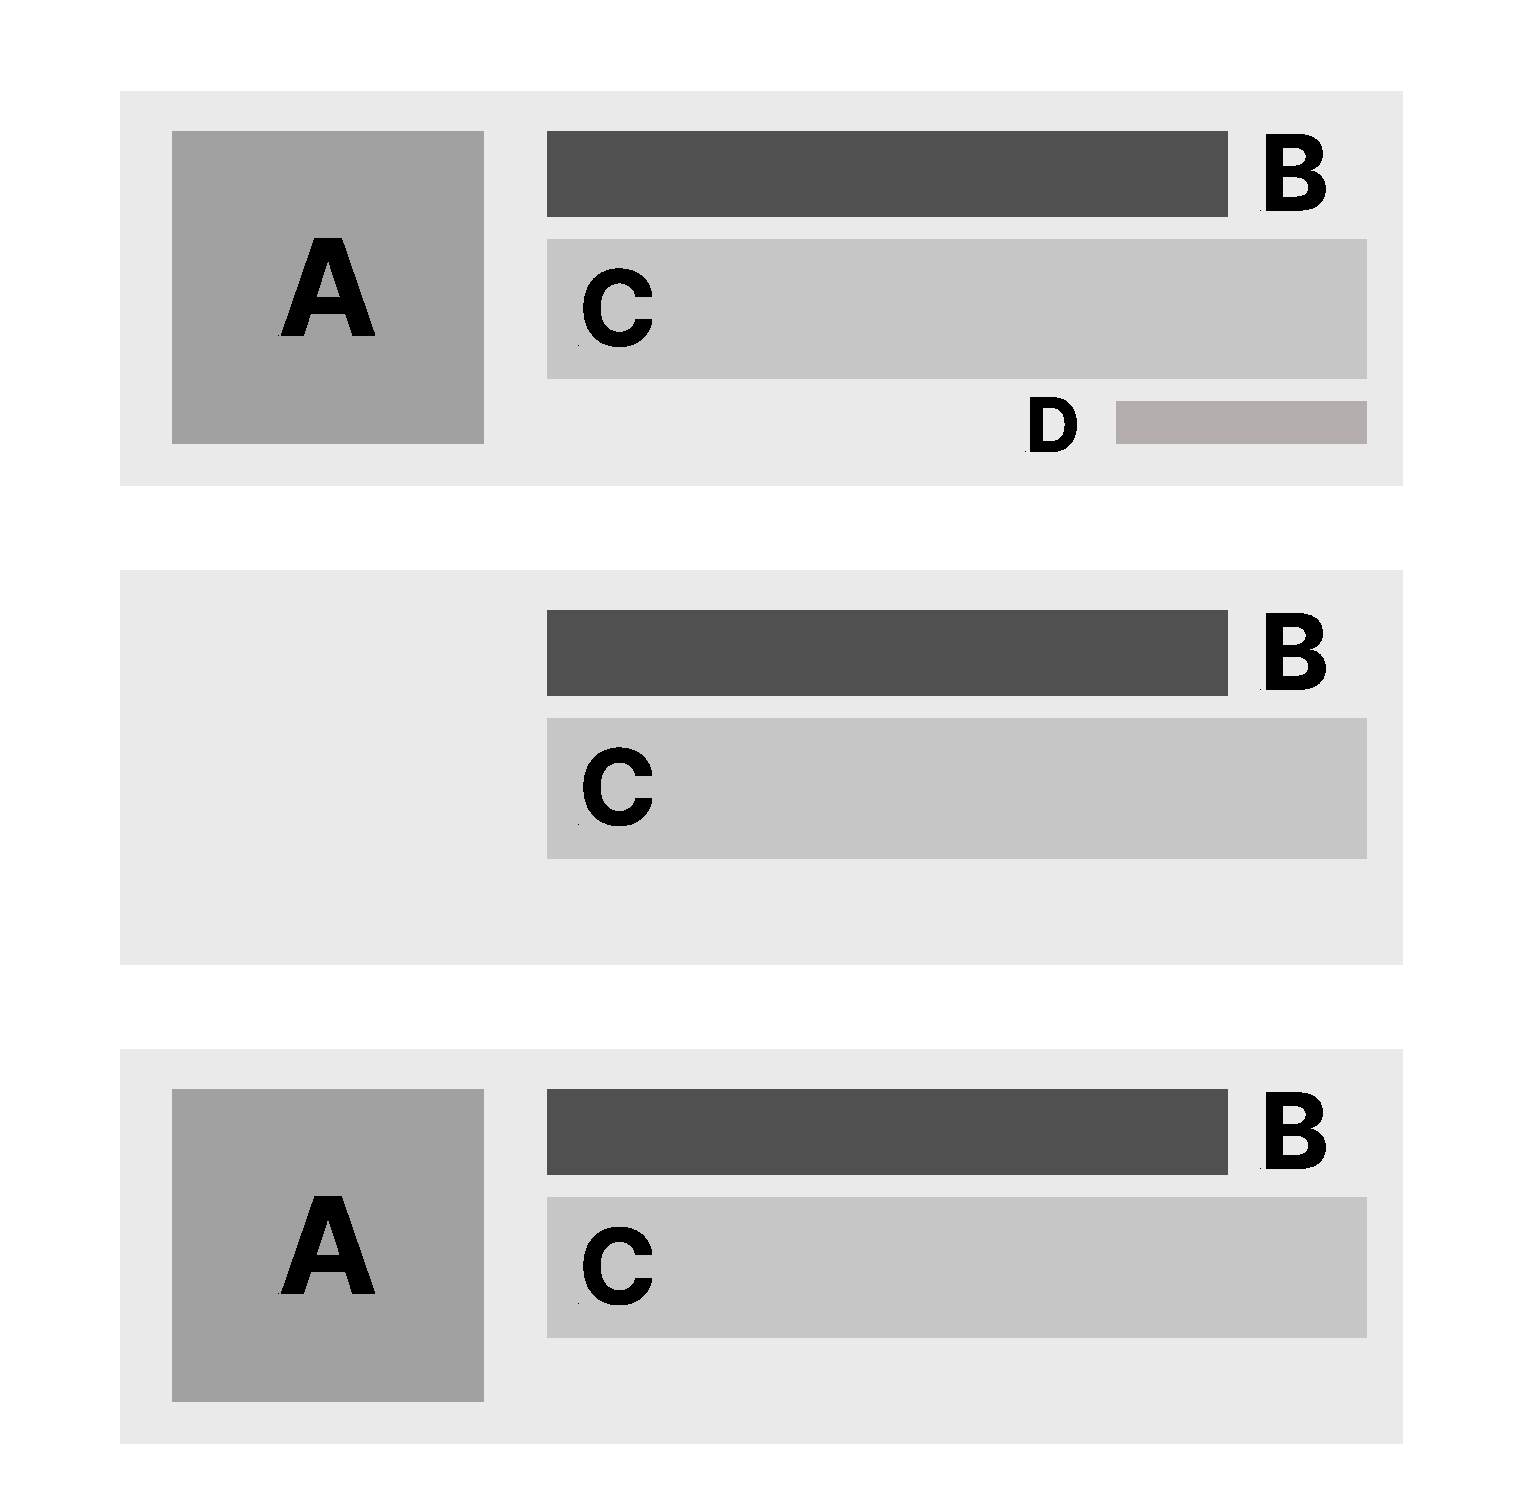
\includegraphics[width=0.4\textwidth]{./img/algos/scrapeSchema.pdf}}
    \end{center}
    \caption{Example page to be scraped}\label{scrapeSchema}
\end{figure}

The \autoref{scrapeSchema} shows an example page containing a table of user profiles. 
A user card can contain a \textit{photo of the user} (A), their \textit{name} (B), their \textit{profile description} (C) and their \textit{phone number} (D).
The letters represent the selectors for the \textit{Runner} to extract the data from.

The user provides the \texttt{scrapeSchema} method with the following schema:
    \begin{lstlisting}[language=json]
                {
                    "photo": "A",
                    "name":  "B",
                    "desc":  "C",
                    "phone": "D"
                }
    \end{lstlisting}

The \textit{Runner} extracts the data from the page. The data is stored in an array of dictionaries, where each dictionary corresponds to a user card.

\begin{lstlisting}[language=json]
[
    {
        "photo": "https://abc.xyz/img/user123.jpg",
        "name":  "John Doe",
        "desc":  "Lorem ipsum dolor sit...",
        "phone": "123-456-7890"
    },
    {
        "photo": undefined,
        "name":  "Mark Smith",
        "desc":  "Ipsum dolor amet sit...",
        "phone": undefined
    },
    {
        "photo": "https://abc.xyz/img/user234.jpg",
        "name":  "Jane Green",
        "desc":  "Sit dolor ipsum lorem...",
        "phone": undefined
    },
]
\end{lstlisting}

Note how the contents of the corresponding elements are paired, leaving the missing fields empty.
This is done by traversing the \acs{DOM} tree of the page, and grouping the elements by their common parents.

\section{Editor}
As described in the \autoref{sec:editor} \textit{Editor}, the workflow editor is implemented as a React Application.
The following section describes decisions made during the implementation of the \textit{Editor} application,
certain problems and their solutions.

% TODO add babel link
% TODO add CRA link
\subsection{React}
While it is possible to set up a \textit{React} application as a plain Node.js application, it is not recommended.
Handling the bundler configuration is cumbersome and requires a respectable amount of knowledge about the React toolchain.
The React's signature \acs{JSX} syntax also requires configuring a transpiler (e.g. \texttt{babel}), which adds another level of complexity.

For those reasons, the \textit{Editor} \textit{React} application has been initialized with \texttt{create-react-app}. 
This is a \ac{CLI} tool for simple initialization of \textit{React} applications.
It mainly provides the \textit{Webpack} and \textit{Babel} configuration files and bootstraps the project with a template website.

\subsubsection{Configuring Webpack polyfills}

For validating the uploaded worklflow files, the \textit{Editor} application imports the \textit{Preprocessor} class from the \textit{Interpret} module.
While both the \textit{Editor} and \textit{Interpret} module are written in \acl{TS}, there are slight differences between \textit{Node.js} and browser code.

% TODO Node.js vs browser modules citation
% TODO react-app-rewired citation
Most of those problems stem from the module resolution, as both \textit{Node.js} and browsers use slightly different approaches to module loading.
While this is covered by Webpack and Babel in most cases, importing the \textit{Interpret} module initially caused errors.

This is because since the version \texttt{5.0.0}, \textit{Webpack} no longer provides polyfills for the core \textit{Node.js} modules, such as \texttt{path} used by the \textit{Interpret} module.
The \texttt{path} module is not used by the validation feature of the \textit{Editor}, so the polyfill could be simply disabled.
However, doing so requires a manual update of the \textit{Webpack} configuration.

Since the \textit{Editor} has been created with \texttt{create-react-app}, the \textit{Webpack} configuration \texttt{webpack.conf.js} is contained in the \verb|node_modules/react-scripts| directory.
While it might be possible to modify the \texttt{webpack.conf.js} file directly, it is not recommended - the \verb|node_modules| directory is used to save all downloaded packages from NPM.
Updating the \texttt{react-scripts} package would then reset all changes made to the configuration file.
Furthermore, because of it's dynamic nature, the \verb|node_modules| directory is ommited from the \texttt{git} version control.

While the official \texttt{create-react-app} guide suggests to perform \texttt{eject}, i.e. to export the configuration files for manual maintenance, this is a borderline unsafe step. 
The \texttt{eject} script performs irreversible changes to the package structure, and forces the user to maintain the configuration and dependencies themselves from then on.

To retain the simplicity of automatic dependency management while still overriding some of the default rules, the solution now uses \texttt{react-app-rewired}.
Published as an \texttt{npm} package, \texttt{react-app-rewired} is an drop-in replacement of \texttt{create-react-app}, which lets the developer to update the configuration files, whlile still maintaining the base configuration.

% \subsubsection{State maintenance}
% % TODO add React.memo link
% One of the biggest features of the \textit{React} framework is the state management and conditional rendering, enabling the developers to create lightweight applications rerendering only the updated \acs{UI} components, instead of redrawing the whole page on any update.

% The first versions of the \textit{Editor} did not take this into consideration and the edited workflow was stored in the top level component, trigerring rerender of all the workflow elements on any update. 
% This was done mainly for the simple consistency maintenance, as keeping the entire workflow in one piece and rerendering all the elements every time ensures that there are no stale elements with old versions of the workflow.

% While this approach did not introduce any measurable performance loss - most probably because of the small total number of rendered elements - in the final version of the \textit{Editor} application, 
% every major component has been wrapped with \texttt{React.memo} - a higher order component allowing memoization of once rendered component and thus theoretically boosting the render performance, since it does not rerender the component if its parameters have not changed.

% One caveat with this solution is that \texttt{React.memo} compares the incoming parameters with shallow equality by default - which is not useful with the hierarchical structures of the workflow definition file.
% For these situations, the \texttt{React.memo} allows the developers to implement own comparison function.

\subsection{Improving the \acs{UX}}
Given the \hyperref[requirements]{nonfunctional requirements} for the \textit{Editor}, the \textit{Editor} application should adhere to the best \ac{UI}/\ac{UX} practices and provide a steep learning curve.
This is manifested multiple times in the \textit{Editor} application itself.


% TODO add react-dnd link
% TODO add react-dnd example link
\subsubsection{Drag \& Drop}
Since the main control elements in the \textit{Editor} are modular blocks, allowing the user to use drag\&drop controls e.g. for reordering the blocks seems like the superior solution in terms of UX.

The drag\&drop feature is used for reordering the blocks in the \textit{Editor} application.
While it would be possible to drag the entire blocks around the application window, it is not recommended due to UX reasons.
This is solved in the \textit{Editor} application by collapsing all the blocks when the drag\&drop action is initiated.
This helps the user to focus on the actual meaning of the reordering action, and not on the content of the blocks.

The implementation of the drag\&drop feature is based on the \texttt{react-dnd} library.
While the authors of this library offer an official example of reordering a list of block elements, the \textit{Editor} implementation is not based on this example due to the mentioned features,
which are not provided by the example solution.

\subsubsection{Argument type suggestions}
The \textit{Editor} application generates a workflow interpretable by the \textit{Runner} application, which is internally using the \textit{Playwright} library.
The function signatures of the workflow reaction steps depend on the \textit{Playwright} library, as most of the supported steps are mirrored from the \texttt{Page} class methods.
While the user might set the types of the arguments themselves, the \textit{Editor} application aims to provide a simple way of creating the web automations.

For this reason, the \textit{Editor} application provides a prefilled list of arguments with the correct types and matching input elements,
which correspond to the \textit{Playwright} \texttt{Page} class methods and present the correct usage of the arguments to the user.
The range of optional arguments is hand-picked for every command to provide the best variability while still maintaining an exceptional level of user-friendliness.


\chapter{Documentation}

The following chapter contains the documentation of the project. 
It is divided into several sections based on the amount of experience of the reader and the desired actions.

\defcitealias{DockerRun}{DockerRef}

\section{Administrator documentation}

The following section contains the administrator documentation of the project.
It contains installation instructions and a short troubleshooting guide for setting up a server for the \textit{Editor} and \textit{Runner} applications. 
It also contains a list of system requirements on the server where the applications are to be deployed

\subsection{Installation instructions}

The \textit{Editor} and \textit{Runner} application are both packaged in the \href{https://www.docker.com/}{Docker} image \texttt{barjin/wbr}.
This Docker image represents a complete server setup, including all the dependencies and the \textit{Editor} and \textit{Runner} applications.

The web server providing the user interface is running on port \texttt{4321} of the Docker container, which is also the only port utilized by the \textit{Editor} and \textit{Runner} applications.

Running the container with the \texttt{barjin/wbr} image then requires only one command:
\begin{verbatim}
    docker run -p 4321:4321 -d barjin/wbr
\end{verbatim}
where \texttt{4321} is the port number used by the \textit{Editor} and \textit{Runner} applications.

The \texttt{-d} option instructs Docker to run the container in so-called `detached mode', which means that the container is not terminated when the command finishes. \citepalias{DockerRun}
In case the user wants to stop the container, they can use the \texttt{docker stop} command with the container ID.

In case the user never ran the \texttt{docker run} nor the \texttt{docker pull} command before, the \textit{Docker daemon} first downloads the \texttt{barjin/wbr} image from the Docker Hub.
Note that this can cause a delay of several seconds and consume a certain amount of bandwidth (ca. TODO MiB).

The Docker image can also be built from the attached Dockerfile by invoking the \texttt{docker build} command in the root folder of the project repository.

\subsection{Build instructions}
Besides the \textit{Docker} image, source files of both applications are also available in the project's GitHub repository. 
The \texttt{package.json} files for the packages \texttt{wbr-interpret} and \texttt{wbr-editor} contain the build instructions for the respective applications,
as well as the required dependencies.

Both packages can be built by invoking the \texttt{npm run build} command in the root folder of the package folders.
After the build process, the tools can be started by calling \texttt{npm start} in the respective package folders.

Please note that building the packages individually is not the recommended way of running the application.
The author of this work holds no responsibility for the results of the build process.

Running the project in the \textit{Docker} container is the recommended way of running the application.
\chapter{Testing}

During the development phase, all parts of the project have been tested using various testing methods.
The following chapter describes the testing methodology and the nature of the individual tests.
Aside from testing the software using automated test suites, user testing was carried out on the \textit{Editor} application.

\section{Code quality}

While the code quality does not directly influence the correctness of the results, it is an important aspect of the project, as it influences readability and maintainability of the code.
Maintaining a consistent code style also speeds up the development process and reduces the risk of introducing bugs.

The \texttt{wbr-interpret} module and the \textit{Editor} application are written in \textit{TypeScript} and \textit{TSX}, respectively.
The codebase of the entire project follows the practices described in the \textit{Airbnb JavaScript Style Guide}\footnote{\href{https://airbnb.io/javascript/}{https://airbnb.io/javascript/}}, made and maintained by \textit{Airbnb, Inc.}
\textit{Airbnb Inc.} also provides a \texttt{.eslintrc} file for configuring \textit{ESLint} in accordance with the practices described in the \textit{Style Guide}.
All the code in the project is then automatically checked for conforming to the style guide using \texttt{ESLint} already during the development phase, which simplifies formatting and allows us to see potential errors right away.

The project's GitHub repository also contains an automated \textit{GitHub Actions} workflow, running the \textit{ESLint} check with every push to the repository.
This helps with catching the bad code patterns early on and prevents the need for further manual testing.

\section{Automated tests}

To ensure the elementary correctness of the project parts, the project has contained automated test suites since the early stage of development.
This helps both with code maintenance and new feature implementation, as the automated test suites ensure we do not introduce any breaking changes.

All of the tests mentioned in the following sections are also ran in the corresponding \textit{GitHub Actions} workflow. 
This ensures that the code available in the main branch of the public repository is always tested against the latest changes.

All the following tests were carried out using the \texttt{jest}\footnote{\href{https://jestjs.io/}{https://jestjs.io/}} testing framework, if not stated otherwise.

\subsection{Unit tests}

The entirety of the \texttt{wbr-interpret} package is covered with unit tests testing the individual components of the package.
Special attention is paid to the \textit{Interpreter} and \textit{Preprocessor} classes, as those are the core of the project
and contain the largest amount of complex code. 

The success of the unit tests is directly related to the code design of the module, 
since almost all methods in both classes were first written as pure functions, and only then they were converted to classes for
encapsulation and to provide a more convenient interface.

\smallskip
While it is possible to unit test components in a React application, most of the components in the \textit{Editor} application are trivial.
For this reason, there are no unit tests for the \textit{Editor} application and all the testing is carried out by \ac{E2E} tests.

\subsection{E2E tests}

Both the \textit{Editor} application and \texttt{wbr-interpret} package have been tested with \acl{E2E} tests as well.
These tests are typically longer and follow a complete user path, testing the entire application from the user's perspective.

The \texttt{wbr-interpret} package is \acl{E2E} tested using custom scripts (not \texttt{jest}) for two different scenarios:
\begin{itemize}
    \item Loading, validating and executing a simple workflow.
    \item Loading, validating, initializing and executing an advanced, parametrized workflow.
\end{itemize}

Both \ac{E2E} tests are run against a local server, which is started before the tests are run.
This way we can observe the actions carried out by the \textit{Runner} even without obtaining any output data.

The \textit{Editor} application has been tested using \textit{Playwright} library to simulate the user's interaction with the application.
There are two tested scenarios:
\begin{itemize}
    \item Uploading various workflow files and seeing which one is valid. 
    \item Creating new automation, editing it, running it, seeing the results and downloading the workflow definition file.
\end{itemize}

All the automations are also run against a local server, which allows us to control the content of the webpages 
and observe the actions caused by the automation execution.

\section{User testing}

Aside from the code testing, the \textit{Editor} application has also been tested by 8 potential users of different technical backgrounds.
This was done in two parts.
First, the users were asked to use the \textit{Editor} application to create a simple automation file.
After getting accustomed to the software, the users were given a \ac{SUS} survey and were asked to rate the application's usability.

\subsection{Test scenario}

The task for the users testing the \textit{Editor} application was to create a simple web automation using the application and execute it to validate the functionality.
Such a task requires utilizing a number of \acs{UI} elements of the \textit{Editor} application, while not being too demanding or requiring much technical knowledge.

\smallskip
The created automation should be able to perform the following steps:
\begin{enumerate}
    \item Navigate to \href{https://jindrich.bar/}{https://jindrich.bar/}.
    \item Click an arbitrary link on the page.
    \item If the resulting page contains paragraphs with text, download these first, otherwise just terminate the execution.
\end{enumerate}
    
The users were provided no additional support during the task.
Out of the eight users, only three of them were able to successfully complete the task, while the others failed at various points.
The successful users were all computer specialists with a strong technical background.
While this might show a trend towards excessive technicality of the application, the sample size is not significant enough to make any conclusions.

The individual user complaints bring better insight into the why some users failed to complete the task.
The less successful users complained mostly about the complexity of the workflow definition format and
the confusing logic of the workflow interpretation.

There were no direct complaints about the application's user interface layout. 
After concluding the experiment, all of the users were instinctively able to find all the control elements when asked to perform a specific action.
All of them were also able to answer questions about the system state.

\subsection{SUS survey}
All the testers have also shared their opinions on the usability of the application via the \ac{SUS} survey.
The detailed results of the \ac{SUS} survey are included in the \hyperref[sec:sussurvey]{Attachment A.1} SUS Survey Results.
The attachment also contains additional information about the survey itself.

The average \ac{SUS} score over the ratings of the eight users is \textbf{52.5}.
This sets the \textit{Editor} application somewhere between the \textit{10th} and \textit{20th} percentile of typical \ac{SUS} evaluated systems.
While this might come off as negative result, it is still a valuable indicator of the quality of the \textit{Editor} application.

The main reasons for the low ratings the users stated were \textit{the workflow definition format being confusing} and the general unfamiliarity with debugging tools. 
While it would be easy to brush these points off as too subjective, the goal of the thesis was to create a tool that would be easy to use and intuitive for the user -
which makes all the user complaints very relevant.
\chapter{Conclusion}

The goal of this work, as stated in the \hyperref[intro]{Introduction} was to \textit{create a human-readable, declarative format for
storing and creating web automations, with an interpreter of this format and a
visual editor, allowing less technical users to create and maintain automations in
this format.}

By implementing the \textit{Editor} application and the \textit{Runner} module, this goal has been achieved in full scale.
Both parts of the project are now fully functional - in accordance with the requirements from the \autoref{requirements} Requiements - and can be used to create and edit web automations
for data extraction and process automation.
Both parts of the project have been developed in a modular fashion, which makes the further development process easier and faster.

Possible future work on the \textit{Editor} application and the \textit{Runner} module is to implement more advanced features.
For instance, less technical users might prefer an automation recorder, implemented as a browser extension.
Such a tool might generate a web automation file in the workflow definition format automatically, without any need for manual editing.
This application might also reuse the components from the \textit{Editor} application to allow for additional workflow editing and inspection.

For more technical users, the debugging features in the \textit{Editor} application could also be further enhanced, as the simplicity of the definition format might allow for more advanced 
analysis features. Such an application might reuse the analysis methods from the \texttt{wbr-interpret} package.

\include{epilog}

%%% Bibliography
\include{bibliography}

%%% Figures used in the thesis (consider if this is needed)
\listoffigures

%%% Tables used in the thesis (consider if this is needed)
%%% In mathematical theses, it could be better to move the list of tables to the beginning of the thesis.
\listoftables

%%% Abbreviations used in the thesis, if any, including their explanation
%%% In mathematical theses, it could be better to move the list of abbreviations to the beginning of the thesis.

\chapwithtoc{List of Abbreviations}

\begin{acronym}
 \acro{GUI}{graphical user interface}
 \acro{RPA}{robotic process automation}
 \acro{QA}{quality assurance}
 \acro{E2E}{end-to-end}
 \acro{SW}{software}
 \acro{UX}{user experience}
 \acro{CORS}{cross-origin resource sharing}
\end{acronym}

%%% Attachments to the bachelor thesis, if any. Each attachment must be
%%% referred to at least once from the text of the thesis. Attachments
%%% are numbered.
%%%
%%% The printed version should preferably contain attachments, which can be
%%% read (additional tables and charts, supplementary text, examples of
%%% program output, etc.). The electronic version is more suited for attachments
%%% which will likely be used in an electronic form rather than read (program
%%% source code, data files, interactive charts, etc.). Electronic attachments
%%% should be uploaded to SIS and optionally also included in the thesis on a~CD/DVD.
%%% Allowed file formats are specified in a provision of the rector no. 72/2017.
\unless\ifdefined\short
	\appendix
	\chapter{Attachments}

	\section{SUS survey details}
	\label{sec:sussurvey}
	This Attachment contains the detailed results of the \ac{SUS} survey for the \textit{Editor} application.
	While the \ac{SUS} is somewhat standardized set of questions for evaluating the quality of software,
	the questions can be updated to match the evaluated software's needs. For completeness, the questions are included in here:
	\begin{enumerate}
		\item I think that I would like to use this application frequently.
		\item I found the application unnecessarily complex.
		\item I thought the application was easy to use.
		\item I think that I would need the support of a technical person to be able to use this application.
		\item I found the various functions in this application were well integrated.
		\item I thought there was too much inconsistency in this application.
		\item I would imagine that people would learn to use this application very quickly.
		\item I found the application very cumbersome to use.
		\item I felt very confident using the application.
		\item I needed to learn a lot of things before I could get going with this application.
	\end{enumerate}
\smallskip
	The response scale for each question is then a 5 point Likert agreement scale:
	\begin{center}
	\begin{tabular}{c | c | c | c | c}
		Strongly disagree &	Disagree & \makecell{Neither agree\\ nor disagree} & Agree & Strongly agree \\
		\hline
1 & 2 & 3 & 4 & 5 \\
	\end{tabular}
	\end{center}

	The results of the evaluees' survey are presented in the following table:
	\begin{center}
		\begin{tabular}{ c | c | c | c | c | c | c | c | c | c | c | c } 
							 & 1 & 2 & 3 & 4 & 5 & 6 & 7 & 8 & 9 & 10 & \textbf{SUS} \\
							 \hline\hline
\textbf{User 1} & \textbf{3} & \textbf{2} & \textbf{4} & \textbf{2} & \textbf{3} & \textbf{2} & \textbf{3} & \textbf{2} & \textbf{4} & \textbf{1} & \textbf{70} \\
\textbf{User 2} & \textbf{2} & \textbf{2} & \textbf{2} & \textbf{3} & \textbf{4} & \textbf{3} & \textbf{2} & \textbf{2} & \textbf{3} & \textbf{2} & \textbf{52.5} \\
\textbf{User 3} & \textbf{4} & \textbf{2} & \textbf{4} & \textbf{2} & \textbf{5} & \textbf{2} & \textbf{4} & \textbf{1} & \textbf{5} & \textbf{2} & \textbf{82.5} \\
\textbf{User 4} & \textbf{3} & \textbf{3} & \textbf{2} & \textbf{4} & \textbf{4} & \textbf{3} & \textbf{3} & \textbf{3} & \textbf{3} & \textbf{4} & \textbf{45} \\
\textbf{User 5} & \textbf{4} & \textbf{2} & \textbf{3} & \textbf{2} & \textbf{4} & \textbf{1} & \textbf{2} & \textbf{2} & \textbf{4} & \textbf{1} & \textbf{72.5} \\
\textbf{User 6} & \textbf{1} & \textbf{3} & \textbf{2} & \textbf{4} & \textbf{3} & \textbf{2} & \textbf{2} & \textbf{3} & \textbf{1} & \textbf{3} & \textbf{35} \\
\textbf{User 7} & \textbf{2} & \textbf{3} & \textbf{2} & \textbf{4} & \textbf{2} & \textbf{3} & \textbf{2} & \textbf{3} & \textbf{2} & \textbf{4} & \textbf{32.5} \\
\textbf{User 8} & \textbf{1} & \textbf{2} & \textbf{2} & \textbf{5} & \textbf{3} & \textbf{3} & \textbf{2} & \textbf{4} & \textbf{1} & \textbf{3} & \textbf{30} \\
\hline
Average & \textbf{2.5} & \textbf{2.4} & \textbf{2.6} & \textbf{3.3} & \textbf{3.5} & \textbf{2.4} & \textbf{2.5} & \textbf{2.5} & \textbf{2.9} & \textbf{2.5} & \textbf{52.5} \\
\end{tabular}
\end{center}

\end{document}
